% \section{JavaScript}

Als JavaScript 1997 veröffentlicht und in den NetScape Navigator integriert wurde, gab es die Bedenken, dass das Öffnen einer Webseite dem Betreiber erlaubt Code auf dem System eines Nutzers auszuführen. Damit dies nicht eintritt, wurde der JavaScript Ausführungskontext in eine virtuelle Umgebung integriert, einer sog. Sandbox \cite{LearningJavaScript}.

Die JavaScript-Sandbox bei Browsern schränkt u. A. den Zugriff auf das Dateisystem ein. Auch Zugriff auf native Bibliotheken oder Ausführung von nativem Code ist nicht möglich \cite{TheSpyInTheSandbox}. Browser bieten darüber hinaus aber einige Schnittstellen an, die es erlauben z. B. Daten beim Client zu speichern oder auch Videos abzuspielen.

\nomenclature[Fachbegriff]{CORS}{Cross-Origin Resource Sharing}
\nomenclature[Fachbegriff]{Ajax}{Asynchronous JavaScript and XML}
\nomenclature[Fachbegriff]{W3C}{World Wide Web Consortium}
\nomenclature[Fachbegriff]{XHR}{XMLHttpRequest}

1999 nahm Microsoft im Internet Explorer 5.0 eine neue Funktion in ihre JavaScript-Umgebung auf: Asynchronous JavaScript and XML (Ajax) \cite{MDNAjax}. Ajax erlaubt die Datenabfrage von Webservern mittels JavaScript. Hierdurch können Inhalte auf Webseiten dynamisch abgefragt und dargestellt werden, wofür zuvor ein weiterer Seitenaufruf notwendig war. Das Konzept wurde kurz darauf von allen damals gängigen Browsern übernommen. Jedoch fand erst mit der Standardisierung von Ajax durch das W3C \cite{TheXMLHttpRequestObject} das Konzept Anklang bei Entwicklern \cite{AngularForEnterpriseReadyWebApplications} \cite{FinkIntroducingSPAs} und ist seitdem der Grundstein für unser dynamisches und interaktives Web \cite{ResearchOnAJAXTechnology}.

Durch dies wurden Webanwendungen immer beliebter, aber Entwickler klagten darüber, dass Browser die Abfragen von JavaScript nur auf dem bereitstellenden Webserver, also \enquote{same-origin}, erlauben \cite{CrossSiteXHRWithCORS}. Um dies zu ermöglichen, wurde im selben Jahr der Standardisierung von Ajax ein erster Entwurf zur Absicherung von Abrufen domänenfremder Ressourcen eingereicht \cite{AuthorizingCORS}, das sogenannte Cross-Origin Resource Sharing.

Über die Jahre wurde der JavaScript-Standard immer umfangreicher, was Entwicklern erlaubte mächtige Werkzeuge sowie Frameworks zu entwickeln, welche die Erstellung von Webanwendungen vereinfachen. Mit Webanwendungen war es nun möglich, einen großen Teil der Funktionalitäten eines Produktes abzubilden. Konzepte, die bei der Implementierung von Webanwendungen beachtet werden müssen, werden nachfolgend erklärt.

% Im folgenden Abschnitt werden, für diese Arbeit relevante, Sicherheitsvorkehrungen von Browsern vorgestellt und beschrieben - darunter auch Cross-Origin Resource Sharing.

%\subsection{Fehleranfälligkeit}
%
%Die Sprache JavaScript stellt an sich auch eine Besonderheit der Umgebung dar. Denn anders als z. B. C, C++, Java gilt sie als fehleranfällig \cite{FastReproducingWebApplicationErrors}. Dies


\subsection{Cross-Origin Resource Sharing (CORS)}

Wie aus der Geschichte zu JavaScript zu sehen ist, entwickelte CORS sich aus dem Wunsch von Entwicklern, nicht auf einen einzelnen Webserver beschränkt zu sein. Diese Einschränkung existierte, um Nutzer vor Missbrauch zu schützen \cite{BrowserProtectionAgainstCSRF}. CORS hebt diese Einschränkung teilweise auf, aber unter Berücksichtigung der sicherheitskritischen Aspekte. Das Konzept von CORS stellt sicher, dass aus einer JavaScript-Umgebung heraus keine Ressourcen von Webservern angefragt werden, welche nicht explizit der Anfrage zustimmen \cite{MDNCORS}.

Wie eine \enquote{cross-origin} Ajax-Anfrage nach dem Konzept von CORS gehandhabt wird, ist in \autoref{fig:cors-workflow} zu betrachten. Wenn eine HTTP-Anfrage nicht \enquote{simple}\footnotemark{} ist, führt der Browser einen sogenannten \enquote{Preflighted Request} aus, bei dem vor der eigentlichen Anfrage eine zusätzliche OPTIONS-Anfrage gesendet wird. Bestätigt nun der Webserver in seiner Antwort auf die OPTIONS-Anfrage, dass die Anfrage so erlaubt ist, wird auch die eigentliche Ajax-Anfrage ausgeführt. Ansonsten schlägt die Anfrage fehl und im JavaScript-Kontext ist lediglich der Fehlschlag zu sehen, ohne einen Hinweis auf die Diskrepanz bzgl. CORS.

\footnotetext{Eine Anfrage ist \enquote{simple}, wenn 1. sie der Methode GET, HEAD oder POST entspricht; 2. sie keine benutzerdefinierten Header enthält; und 3. der \enquote{Content-Type} von POST-Anfragen einem der folgenden Werte entspricht: \enquote{application/x-www-form-urlencoded}, \enquote{multipart/form-data} oder \enquote{text/plain} \cite{MDNCORS}.}

\begin{figure}[H]
	\centering
	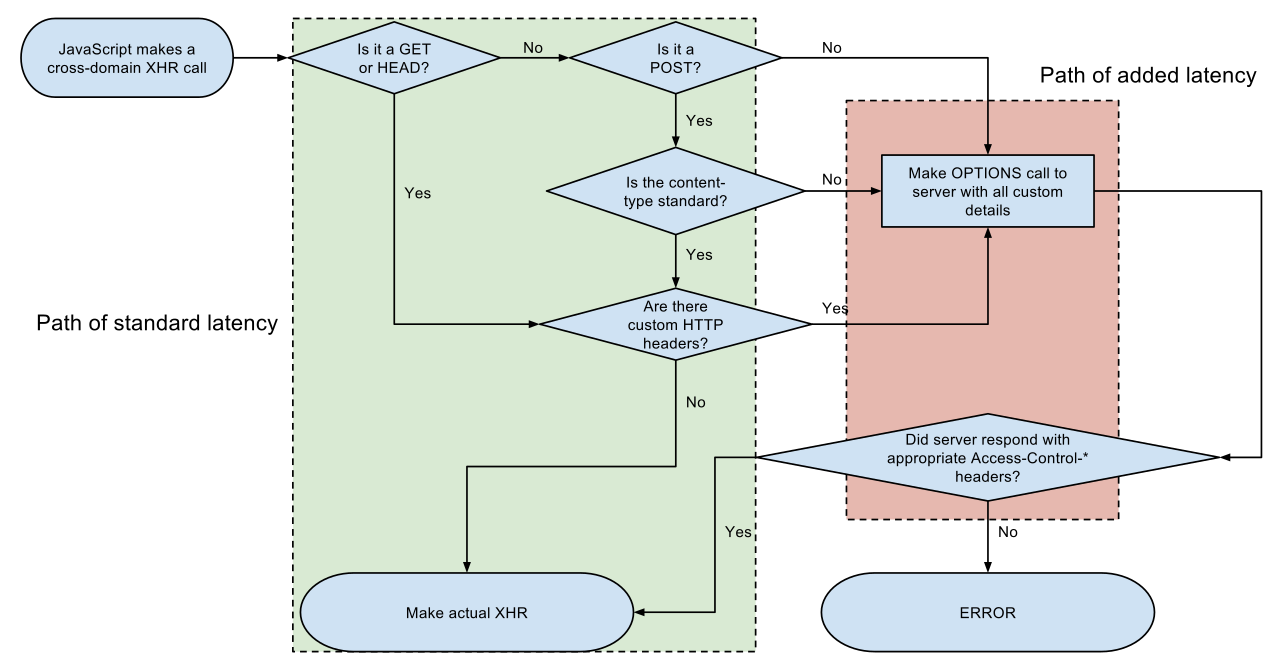
\includegraphics[width=\linewidth]{img/02_theorie/1280px-Flowchart_showing_Simple_and_Preflight_XHR.svg.png}
	\caption{Flowchart über den Ablauf von Ajax-Anfragen mit CORS \cite{FlowchartCORS}}
	\label{fig:cors-workflow}
\end{figure}

\subsection{Content-Security-Policy}

\nomenclature[Fachbegriff]{CSP}{Content-Security-Policy}
\nomenclature[Fachbegriff]{XSS}{Cross-Site-Scripting}
\nomenclature[Fachbegriff]{CDN}{Content Delivery Network}

Neben CORS gibt es im Browser eine Möglichkeit zu bestimmen, welche Funktionalitäten einer Webanwendung zur Verfügung stehen und wie diese vom Browser einzuschränken sind. Diese Funktion heißt Content-Security-Policy (CSP) und dient unter anderem dem Schutz vor Cross-Site-Scripting, indem eine Webanwendung beschränken kann, welche Funktionalitäten in JavaScript verfügbar sind und von wo aus Skripte und Daten geladen werden dürfen \cite{MDNContentSecurityPolicy}. Weiterhin kann bei einem Versuch diese Regeln zu umgehen, eine Berichterstattung darüber eingerichtet werden.